\section{Experiment}
\label{sec:exp}
To investigate \textbf{Q2} and \textbf{Q3}\footnote{See section \ref{sec:method}} an experiment is conducted, utilizing the evaluation framework DocTide Labs as described in section \ref{sec:eval}. 
\\ \\
The evaluation is conducted using the opensource repository \textcolor{red}{Repository samt motivation for hvorfor dette repository er valgt.} A slice of the commit history ranging from \textcolor{red}{valgte commits} has been used as the commits to replicate during the evaluation.

Two metrics is collected through this experiment: \textit{'semantic similarity} and \textit{'success rate'}.

\textcolor{red}{Skulle 'success rate' som metric måske omdøbes til 'format reliability', bpde her og i method? Og så ville denne bare blive introduceret i method som en success metric hvilket er en type fra wangs evaluerings afsnit.}


\subsection{Semantic Similarity}
Through the experiment when the DocTide agent generate documenation for a piece of code that has original documentation generated by a human developer, these pairs of documentation is collected. The Python module Sentence Transformers\footnote{\url{https://www.sbert.net/examples/cross_encoder/applications/README.html}} is then used to calculate the semantic similarity through running a Cross Encoder model.

Taking into considerations the efficiency of running this model over large quantities of comment pairs, we have decided to use the \textit{'stsb-roberta-base'} model, which scores 90.17 in the STSbenchmark\footnote{\url{https://sbert.net/docs/cross_encoder/pretrained_models.html}}.
\subsubsection{Identifying thresholds}
Running the experiment resulted in the collection of 177 unique sets of comment pairs and their semantic score, the distribution of which is seen in \cref{fig:sem_hist}.
\begin{figure}[H]
\centering
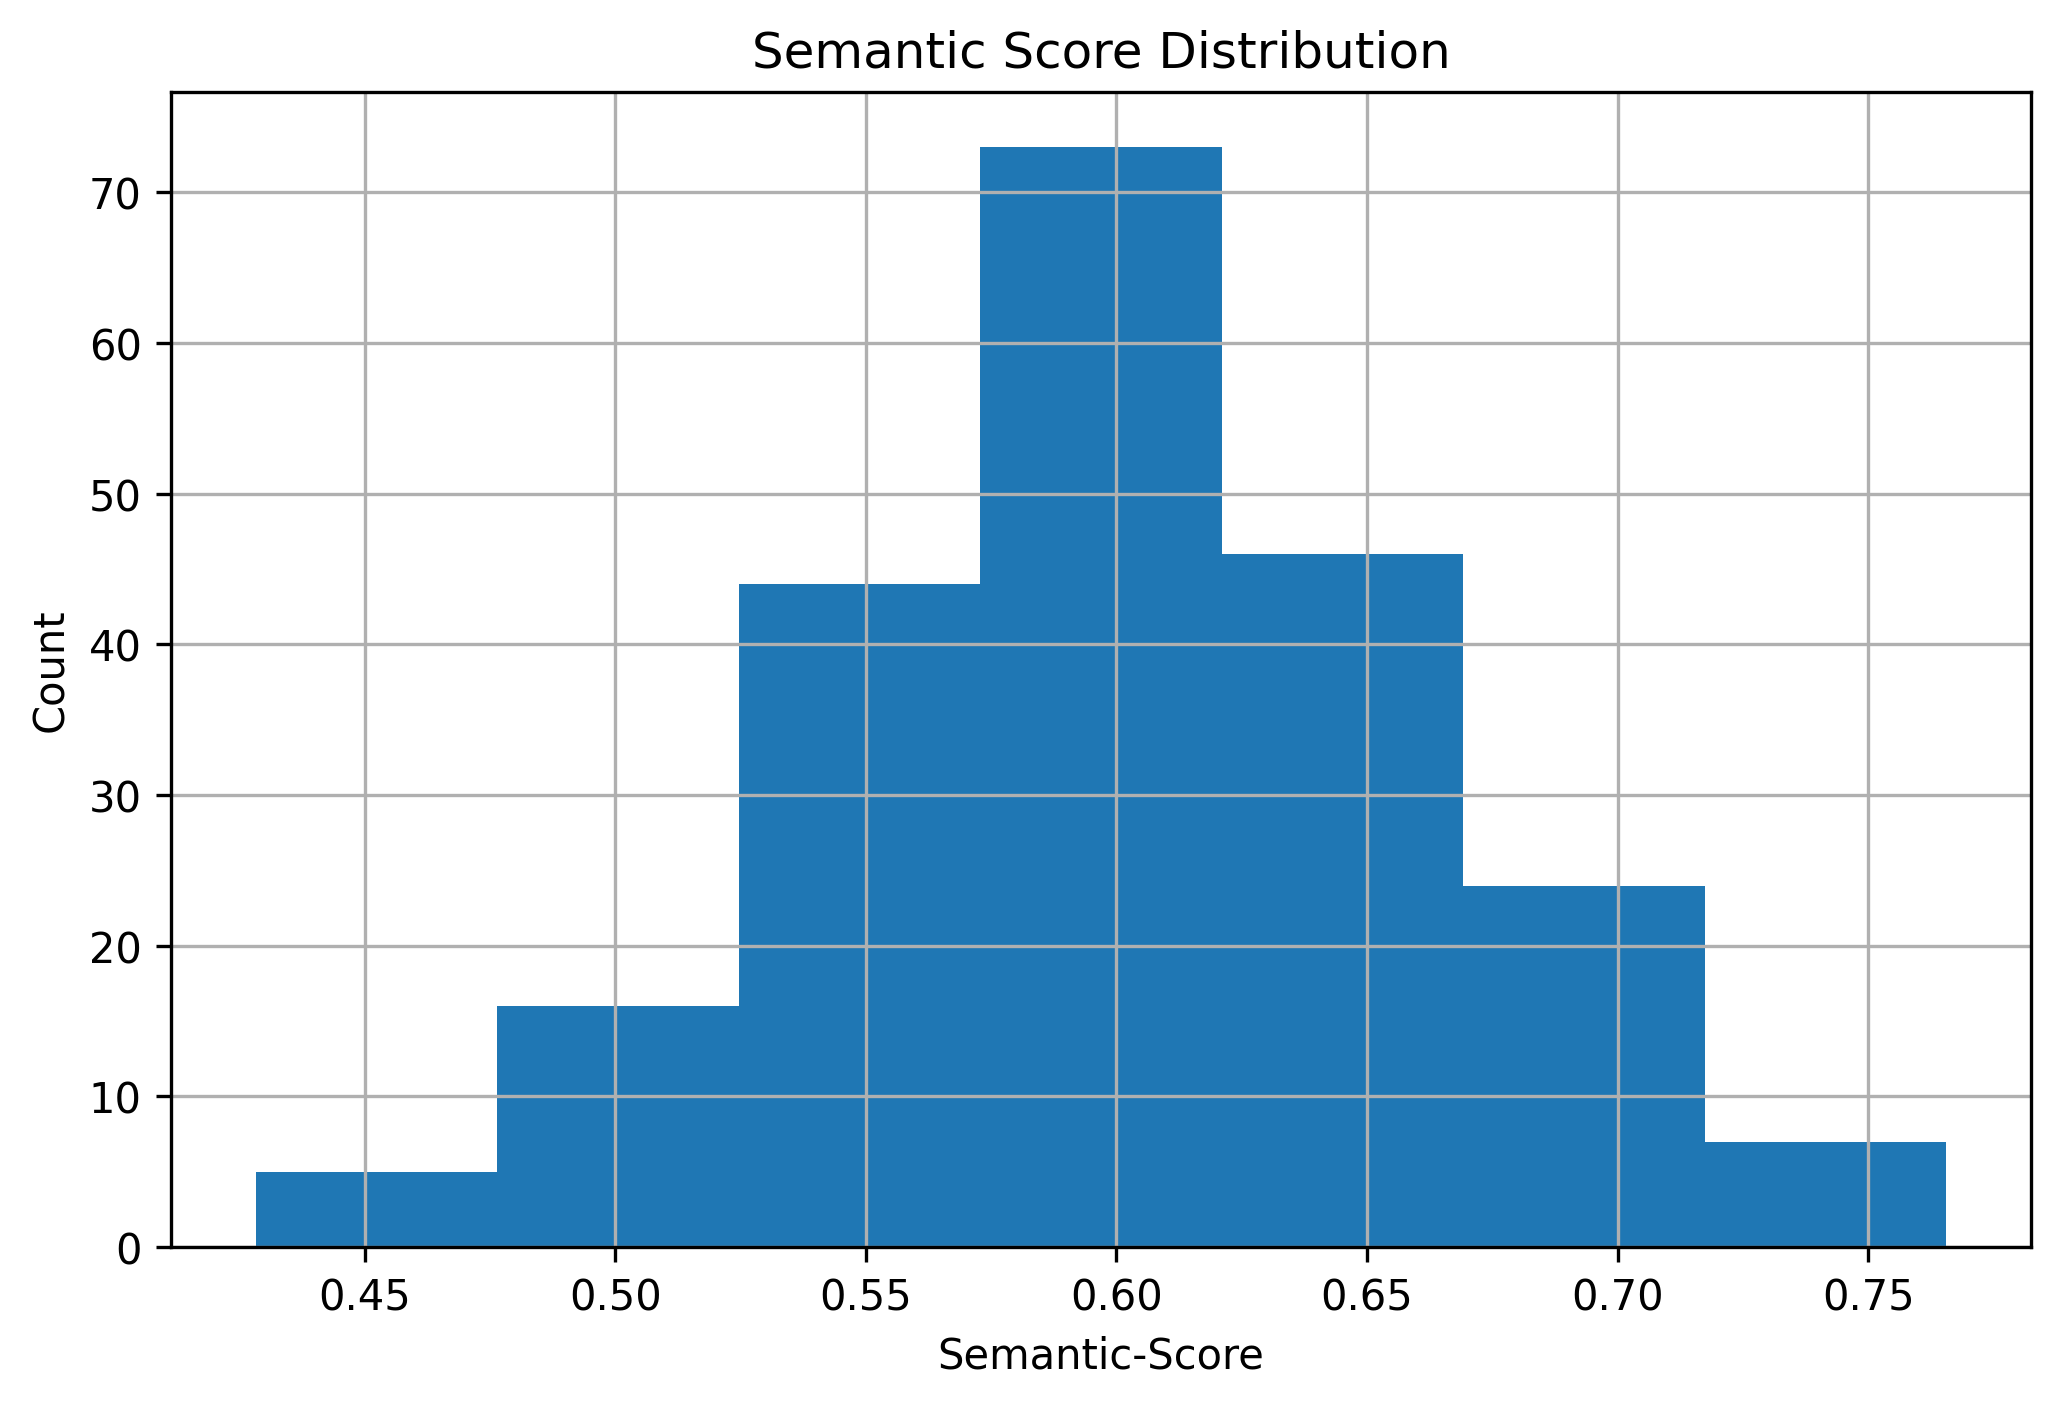
\includegraphics[width=0.7\linewidth]{Figures/semantic_score_histogram.png}
\caption{Histogram showing the normal distribution of the semantic-score metric collected}
\label{fig:sem_hist}
\end{figure}

Before being able to infer any information from this result, the result is processed in order to qualitatively identify what merits as a \textit{'good'} score in semantic similarity. The three quality buckets \textit{'Low-'}, \textit{'Medium-'} and \textit{'High similarity'}, and the thresholds between these is identified as follows:
\\\\
First a \textbf{sample} is taken from the result pairs, which all contain the original comment, the agent generated comment and the semantic score. As \cref{fig:sem_hist} shows the results following a normal distribution, the \textbf{sample} is taken to be representing by utilizing \textit{stratified sampling}\footnote{\url{https://www.geeksforgeeks.org/stratified-sampling-in-pandas/}}. The column containing the semantic score is then disabled, and each pair is qualitatively inspected by comparing the original comment to the agent generated comment, before finally being assigned to one of the three buckets described above. 

Next the \textbf{sample} is grouped by the assigned buckets, and summary statistics is calculated as seen in \textcolor{red}{Indsæt tabel over dette efter labeling stadie} and finally the thresholds is then calculated by summing the first and third quartile from the higher and lower bucket respectively.:
\[
Low\_to\_medium = \frac{Q1_{medium}+Q3_{low}}{2} = \textcolor{red}{???}
\]
\[
Medium\_to\_high = \frac{Q1_{high}+Q3_{medium}}{2} = \textcolor{red}{???}
\]

\subsubsection{Results}
In \cref{fig:sem_box} the results of the experiment is plotted against the quality thresholds identified above. Out of the 117 datapoints collected, \textcolor{red}{Skriv hvordan de ligger i forhold til thresholds med outliers, quantiles osv. - Venter på labeling}

\label{sec:sem_results}
\begin{figure}[H]
\centering
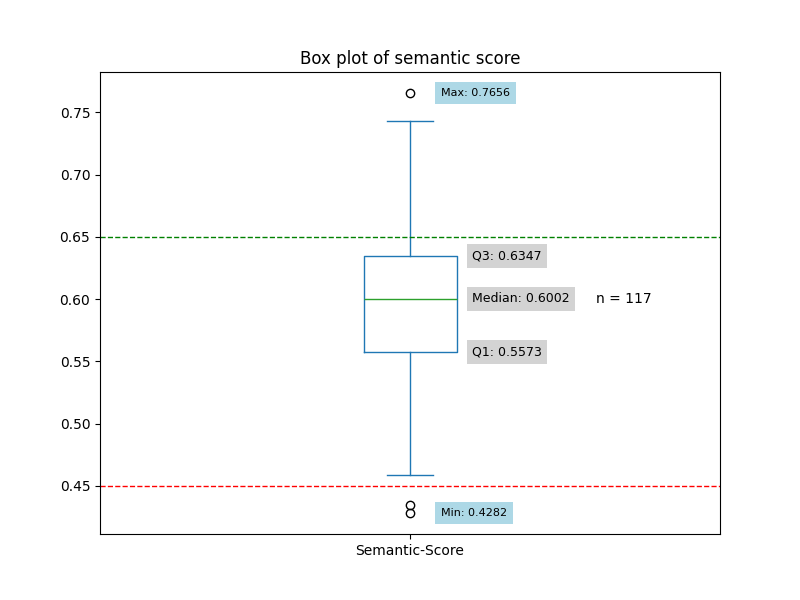
\includegraphics[width=0.7\linewidth]{Figures/semantic_score_box_plot.png}
\caption{Box plot showing the summary-statistics of the semantic scores. The threshold \textit{Low\_to\_medium} and \textit{Medium\_to\_high} is indicated by the red and green line respectively. \textcolor{red}{Remember to insert correct plot after labeling}}
\label{fig:sem_box}
\end{figure}

\subsection{Reliability}
When running the DocTide agent with the 'testing' flag set to true, a success rate is collected for how many attempts ends with the agent generating documentation in the correct format.
Through the experiment, this is collected by a validation function \textit{validate\_response\_as\_comment()}, which is run for every response created. This function analyses the response from the LLM by creating a AST of the response using Tree-sitter\footnote{\url{https://tree-sitter.github.io/tree-sitter/}}, and then check that all nodes is of type comment.
We calculate the score by counting all successful formatted responses and all possible responses and then simply calculate the ratio between those two numbers.
\subsubsection{Reliability results}
\label{sec:suc_results}

Due to an error in the data-formatting during the experiment, the reliability metric was only collected for the commits in the ranges \textit{HEAD\textasciitilde366}-\textit{HEAD\textasciitilde300} and  \textit{HEAD\textasciitilde200}-\textit{HEAD\textasciitilde114}. \textcolor{red}{Tjek at range er rigtig, og hvad synes vi om denne tilde?}
\\ \\
During these commits the DocTide agent attempted to generate \textbf{315} times, out of which \textbf{216} were in the correct format. This means that 216 times the generated DocTide was able to re integrate the generated comment into the code. This corresponds to a success\_rate of:
\[
Success\_rate=\frac{216}{315}*100\% = 68.57\%
\]

\subsection{Limitiations / Threats to validity}
The notion of success that we described in the method \Cref{sec:method} was build on knowledge obtained in the early stage of development, when we encountered that the LLM returned comments in markdown format, with the function definition at the beginning, with explanatory comments on what it has made, all formats which is not integrable into source code. Therefor we constructed this measurement of success based on the agents ability to generate documentation which would be integrable.
A potential thread to the construct validity of the semantic metric, is that if the developers function-level document is purely descriptive and does not embed human level intent, then is is not a measurement for DocTides human behavior, but on its ability to describe the code. One of the limitation of the the level of intent DocTide is able to show is the level of build in intent in the function source code, since it does not have any other content then that. Some errors which were thrown under the execution of the testing framework has not been resolved:
\begin{lstlisting}[language=bash, label={lst:unresolved_errors}, caption=Unresloved errors ]
    github.GithubException.UnknownObjectException: 404 {"message": "Not Found", "documentation_url": "https://docs.github.com/rest/repos/contents#get-repository-content", "status": "404"}
\end{lstlisting}

\textcolor{red}{Brainstorm: \begin{itemize}
    \item Thread to construct validity: Semantisk similarity sammenligner det med udvikler, det er godt da vi gerne vil immitere menneskelige evner for vores agent, men hvad hvis den originale documentation er dårlig? Måske tvilsomt, hvis vi bare holder os til at målet er at det skal have SAMME nivea som udviklere.
    \item Måske mere relevant er, vi får kun et datapunkt hvis der er original dokumentation. Hvad hvis de originale udviklere har været meget konservative med hvor de vil skrive dokumentation. Måske dette også åbner for snakken om at vi derfor siger at vi vil måle evnen til at 'generate dokumentation with same capabilities as a human developer", men vi måler ikke på den del af capabilities som er at vurdere hvor kode skal dokumenteres. Dette er noget vi ikke kan sige noget om baseret på vores data.
    \item Intent - Hvis ikke udviklere har været gode til at skrive intent ind i koden, så vil den aldrig kunne finde denne information, det kan føre til laverer scores.
\end{itemize}}